% Комбинирование векторных масок.
\subsection{Векторизация с объединением и комбинированием масок}

В общем случае можно считать, что в результате слияния под соответствующими предикатами ветвей исполнения внутри тела плоского цикла мы получим совокупность векторных блоков, обрабатывающихся сходим образом: загрузка входных данных \texttt{in\_data} под маской векторного блока, выполнение вычислений \texttt{block} под маской блока, сохранение результатов \texttt{out\_data} под маской блока (см. рис.~\ref{fig:text_4_vec_comb_mask_vec_block}).
На этой схеме \texttt{in\_data} и \texttt{out\_data} могут являться как одиночными векторами, так и наборами векторов.

\begin{figure}[ht]
\centering
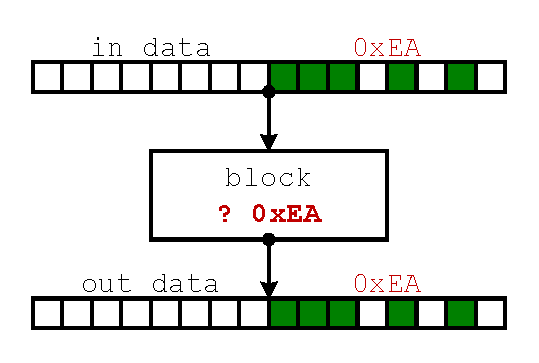
\includegraphics[width=0.5\textwidth]{./pics/text_4_vec_comb_mask/vec_block.pdf}
\singlespacing
\captionstyle{center}\caption{Схема вычислений векторизованного блока команд с входными данными \texttt{in\_data}, выходными данные \texttt{out\_data} и маской исполнения \texttt{0xEA}.}
\label{fig:text_4_vec_comb_mask_vec_block}
\end{figure}

Проверка маски блока на пустоту может повысить эффективность кода, если маски часто оказываются пустыми.
Однако этот никак не поможет в том случае, если в маске выставлено несколько битов.
В некоторых случаях достичь повышения производительности можно путем объединения двух соседних векторных блоков \cite{Rybakov2024VecComb}.

\subsubsection{Объединение непересекающихся масок}

Если у нас есть два соседних векторных блока \texttt{in\_data\_1} $\rightarrow$ \texttt{block} $\rightarrow$ \texttt{out\_data\_1} и \texttt{in\_data\_2} $\rightarrow$ \texttt{block} $\rightarrow$ \texttt{out\_data\_2}, которые должны выполняться под разными векторными масками\label{term:vector_mask5} \texttt{mask\_1} и \texttt{mask\_2}, и в дополнение к этому для этих масок выполнено условие \texttt{(mask\_1 \& mask\_2) == 0x0} (то есть маски не пересекаются), то вычисление этих двух соседних блоков можно объединить.\label{term:meth_vec_union}
Вместо последовательного выполнения двух векторных блоков можно объединить входные данные \texttt{in\_data\_1} и \texttt{in\_data\_2} с помощью слияния \texttt{in\_data = \_mm512\_mask\_blend\_ps(mask\_1, in\_data\_2, in\_data\_1}), после чего выполнить тот же блок вычислений под маской \texttt{mask\_1 | mask\_2}.
Ввиду отсутствия пересечения векторных масок в результирующих выходных данных \texttt{out\_data} будут содержаться как необходимые элементы данных \texttt{out\_data\_1}, так и необходимые элементы данных \texttt{out\_data\_2}.
Последним действием, которое нужно выполнить является извлечение из объединенного результата \texttt{out\_data} данных \texttt{out\_data\_1} и \texttt{out\_data\_2} (см. рис.~\ref{fig:text_4_vec_comb_mask_comb_masks}).

\begin{figure}[ht]
\centering
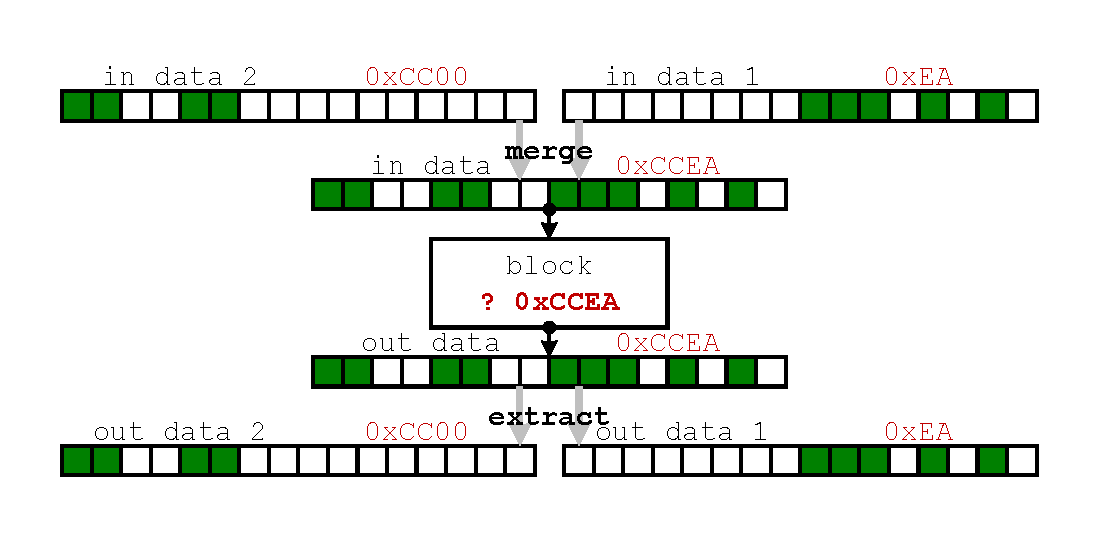
\includegraphics[width=1.0\textwidth]{./pics/text_4_vec_comb_mask/comb_masks.pdf}
\singlespacing
\captionstyle{center}\caption{Схема вычислений с объединением двух векторизованных блоков \texttt{in\_data\_1} $\rightarrow$ \texttt{block} $\rightarrow$ \texttt{out\_data\_1}, \texttt{in\_data\_2} $\rightarrow$ \texttt{block} $\rightarrow$ \texttt{out\_data\_2}.
Объединение допустимо, так как векторные маски \texttt{0xCC00} и \texttt{0xEA} не пересекаются, объединенный блок выполняется под маской \texttt{0xCCEA}.}
\label{fig:text_4_vec_comb_mask_comb_masks}
\end{figure}

В результате такого преобразования в случае отсутствия пересечения векторных масок количество вычислений рассматриваемого блока \texttt{block} сокращается вдвое, а плотность векторных масок\label{term:vector_mask_density2} внутри блока повышается.
Однако вместе с этим появляются накладные расходы, связанные с проверками масок, а также операции слияния данных до вычислений блока и выделения нужных данных после вычислений.
Заметим, что эту технику можно применять для объединения трех и более соседних блоков, однако это связано с еще большим возрастанием накладных расходов.

\subsubsection{Комбинирование пересекающихся масок}

\label{term:meth_vec_comb}Еще один подход, о котором стоит упомянуть, но который не проверялся с точки зрения эффективности, связан с объединением соседних блоков с пересекающимися масками, то есть для которых \texttt{(mask\_1 \& mask\_2) != 0x0}.

\begin{figure}[ht]
\centering
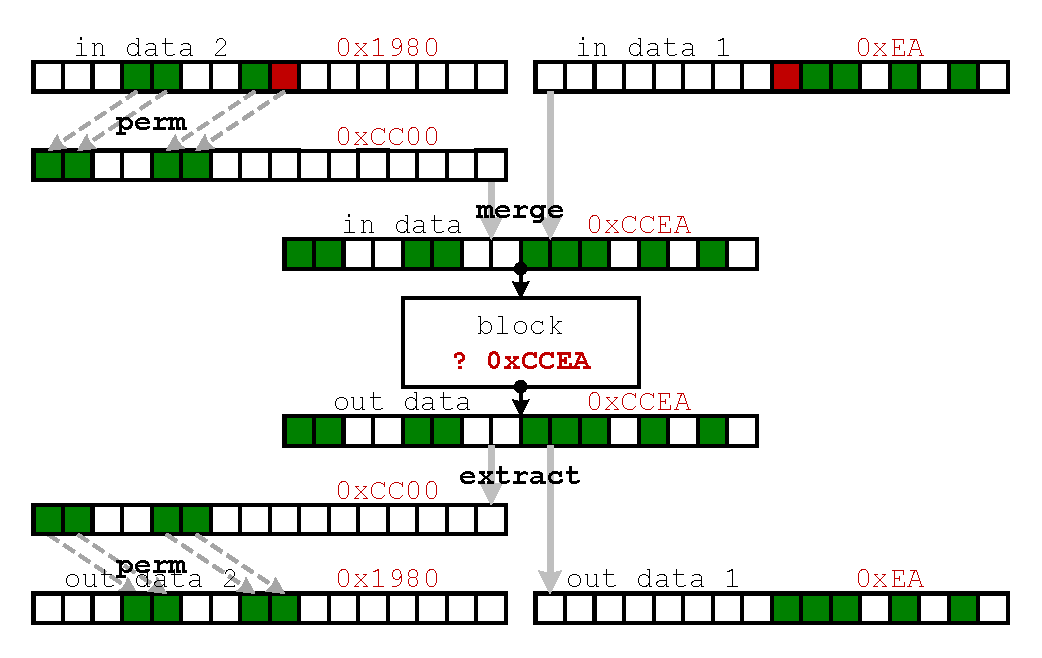
\includegraphics[width=1.0\textwidth]{./pics/text_4_vec_comb_mask/comb_masks_perm.pdf}
\singlespacing
\captionstyle{center}\caption{Схема вычислений с объединением двух векторизованных блоков при условии пересечения их масок. Для объединения применяется техника изменения порядка элементов в данных одного из блоков.}
\label{fig:text_4_vec_comb_mask_comb_masks_perm}
\end{figure}

Если мы имеем дело с двумя масками низкой плотности, которые пересекаются, но для которых выполнено условие непревышения суммарной плотности ширины векторизации\label{term:vec_shir3} \texttt{popcnt(mask\_1) + popcnt(mask\_2) <= w}, то такие блоки также можно объединить.
Для этого перед объединением необходимо применять преобразование одной или обеих масок.

\begin{definition}
Преобразование \texttt{perm\_to} векторной маски\label{term:vector_mask6} \texttt{mask} называется обратимым\label{term:obratim_preobr}, если существует преобразование \texttt{perf\_from} такое, что \texttt{perm\_from(perm\_to(mask)) = mask}.
\end{definition}

Для выполнения комбинирования векторных масок двух соседних блоков необходимо найти обратимое преобразование одной из масок (например, \texttt{mask\_1}) \texttt{perm\_to} такое, что будет выполнено условие \texttt{(perm\_to(mask\_1) \& mask\_2) == 0x0}.
В этом случае элементы входных данных переставляются местами в соответствии с преобразованием \texttt{perm\_to}, применяется описанная выше техника объединения блоков, а для выходных данных выполняется перестановка элементов в соответствии с преобразованием \texttt{perm\_from} (см. рис.~\ref{fig:text_4_vec_comb_mask_comb_masks_perm}).

В описанном подходе следует отметить следующие моменты.
Во-первых, объединять можно не только два соседние блока, но также три и более, хотя это существенно усложняет программный код и увеличивает количество накладных расходов.
Во вторых, следует принимать во внимание доступные операции по изменению порядка расположения элементов векторов, так как таких операций достаточно много и они отличаются по времени выполнения (SHUF, UNPCK, VPERM, VPERMIL и другие).
Ну и наконец преобразование исходных масок можно применять не к одной из них, а сразу к обеим маскам.
В этом случае необходимо найти обратимое преобразование первой маски \texttt{perm\_to\_1} и обратимое преобразование второй маски \texttt{perm\_to\_2}, такие что будет выполнено условие \texttt{(perm\_to\_1(mask\_1) \& perm\_to\_2(mask\_2)) = 0x0}.

\subsubsection{Анализ эффективности применения объединения \\ векторных масок}\label{sec:text_4_comb_mask_analyze}

В качестве примера, на котором проводился анализ эффективности векторизации плоских циклов с использованием объединения непересекающихся масок соседних векторизованных блоков, рассмотрим одну из функций реализации газодинамического римановского решателя\label{term:riemann_solver4} -- функцию \texttt{prefun}.
Для удобства будем пользоваться реализацией этой функции на языке программирования C \cite{riemannvecGithub}, как это представлено на листинге~\ref{lst:text_4_vec_comb_prefun_scalar}.

\begin{singlespace}
\begin{lstlisting}[caption={Скалярная версия функции \texttt{prefun} из состава \\ римановского решателя.},label={lst:text_4_vec_comb_prefun_scalar}]
void scase_prefun_1(float& f, float& fd,
                    float p, float dk, float pk, float ck)
{
    if (p <= pk)
    {
        float prat = p / pk;
        f = riemann::sg4 * ck * (pow(prat, riemann::sg1) - 1.0f);
        fd = (1.0f / (dk * ck)) * pow(prat, -riemann::sg2);
    }
    else
    {
        float ak = riemann::sg5 / dk;
        float bk = riemann::sg6 * pk;
        float qrt = sqrt(ak / (bk + p));
        f = (p - pk) * qrt;
        fd = (1.0f - 0.5f * (p - pk) / (bk + p)) * qrt;
    }
}
\end{lstlisting}
\end{singlespace}

На листинге~\ref{lst:text_4_vec_comb_prefun_scalar} мы видим реализацию функции \texttt{prefun}, обрабатывающей один набор скалярных данных.
Функция принимает на входные аргументы \texttt{p}, \texttt{dk}, \texttt{pk}, \texttt{ck} и вычисляет выходные аргументы \texttt{f}, \texttt{fd}.
Функция содержит одно условие в зависимости от которого вычисляются выходные аргументы.
Стоит отметить, что обе ветви исполнения содержат достаточно тяжелые вычисления (содержат операции вещественного деления, извлечения квадратного корня и возведения в степень), что делает оправданным применение проверки масов на пустоту.
Все задействованные в реализации функции операции имеют векторные аналоги в наборе инструкций AVX-512 (точнее в наборе функций-интринсиков\label{term:intrinsic3}), поэтому приведенная функция может быть векторизована путем замены скалярных операций векторными аналогами и слияния ветвей исполнения под соответствующими предикатами, как это показано на листинге~\ref{lst:text_4_vec_comb_prefun_vec}.

В процессе векторизации умышленно не применялись никакие локальные оптимизации, все скалярные операции были строго заменены на векторные аналоги с сохранением порядка вычислений с точности до ассоциативности умножения.
Для удобства код, относящийся к блокам \texttt{block A} и \texttt{block B}, заключен в фигурные скобки.

\begin{singlespace}
\begin{lstlisting}[caption={Векторизованная версия функции \texttt{prefun} из состава римановского решателя.},label={lst:text_4_vec_comb_prefun_vec}]
void vcase_prefun_1(__m512& f, __m512& fd,
                    __m512& p, __m512& dk, __m512& pk, __m512& ck,
                    __mmask16 m)
{
  __mmask16 cond = _mm512_kand(_mm512_cmple_ps_mask(p, pk), m);
  __mmask16 ncond = _mm512_kand(_mm512_knot(cond), m);

  { // first branch
    __m512 prat = _mm512_mask_div_ps(zero, cond, p, pk);
    f = _mm512_mask_mul_ps(f, cond,
          _mm512_mask_mul_ps(zero, cond, riemann::g4, ck),
          _mm512_mask_sub_ps(zero, cond,
            _mm512_mask_pow_ps(zero, cond, prat, riemann::g1),
            one));
    fd = _mm512_mask_mul_ps(fd, cond,
           _mm512_mask_div_ps(zero, cond, one,
             _mm512_mask_mul_ps(zero, cond, dk, ck)),
           _mm512_mask_pow_ps(zero, cond, prat,
             _mm512_mask_sub_ps(zero, cond, zero, riemann::g2)));
  }
  { // second branch
    __m512 ak = _mm512_mask_div_ps(zero, ncond, riemann::g5, dk);
    __m512 bk = _mm512_mask_mul_ps(zero, ncond, riemann::g6, pk);
    __m512 qrt = _mm512_mask_sqrt_ps(zero, ncond,
                   _mm512_mask_div_ps(zero, ncond, ak,
                     _mm512_mask_add_ps(zero, ncond, bk, p)));
      f = _mm512_mask_mul_ps(f, ncond,
            _mm512_mask_sub_ps(zero, ncond, p, pk), qrt);
      fd = _mm512_mask_mul_ps(fd, ncond,
             _mm512_mask_sub_ps(zero, ncond, one,
               _mm512_mask_mul_ps(zero, ncond, half,
                 _mm512_mask_div_ps(zero, ncond,
                   _mm512_mask_sub_ps(zero, ncond, p, pk),
                   _mm512_mask_add_ps(zero, ncond, bk, p)))),
             qrt); 
  }
}                 
\end{lstlisting}
\end{singlespace}

Сравнивая листинги \ref{lst:text_4_vec_comb_prefun_scalar} и \ref{lst:text_4_vec_comb_prefun_vec}, содержащие скалярный и векторный код, можно установить соответствие между участвующими в них объектами, как это показано в таблице~\ref{tbl:text_4_vec_comb_prefun_obj}.

\begin{table}
\centering
\singlespacing
\captionstyle{center}\caption{Соответствие скалярных и векторных объектов \\ листингов \ref{lst:text_4_vec_comb_prefun_scalar} и \ref{lst:text_4_vec_comb_prefun_vec}.}
\bigskip
\label{tbl:text_4_vec_comb_prefun_obj}
\begin{tabular}{ | c | c | }
  \hline
  Скалярный объект & Векторный объект \\ \hline\hline
  \makecell{скалярные аргументы \\ \texttt{float f}, \texttt{fd}, \texttt{p}, \texttt{dk} ...} & \makecell{векторные аргументы \\ \texttt{\_\_m512 f}, \texttt{fd}, \texttt{p}, \texttt{dk} ...} \\ \hline
  \makecell{скалярные глобальные данные \\ \texttt{riemann::sg1}, \texttt{riemann::sg2} ...} & \makecell{векторные глобальные данные \\ \texttt{riemann::g1}, \texttt{riemann::g2} ...} \\ \hline
  \makecell{скалярные операции \\ \texttt{+}, \texttt{-}, \texttt{*}, \texttt{\/}, \texttt{pow}} & \makecell{векторные команды, \\ заданные функциями-интринсиками \\ \texttt{\_mm512\_mask\_[add/sub]\_ps}, \\ \texttt{\_mm512\_mask\_[mul/div]\_ps}, \\ \texttt{\_mm512\_mask\_pow\_ps}} \\ \hline
  \makecell{скалярная операция сравнения \\ \texttt{<=}} & \makecell{векторные операции получения масок \\ \texttt{\_mm512\_cmple\_ps\_mask}, \\ \texttt{\_mm512\_knot}, \texttt{\_mm512\_kand}} \\ \hline
\end{tabular}
\end{table}

Из приведенного на листинге~\ref{lst:text_4_vec_comb_prefun_vec} векторного кода видно, что часть команд выполняется с использованием векторной маски \texttt{cond}, тогда как другая часть команд использует векторную маску \texttt{ncond}.
При этом понятно, что если маска cond окажется нулевой, то нет необходимости выполнять инструкции, использующие эту маску.
То же касается маски \texttt{ncond}.
Для того, чтобы учесть это изменение достаточно перед выполнением блока операций, относящихся к \texttt{block A}, проверить маску cond на пустоту, в противном случае вообще не выполнять соответствующие инструкции.
Аналогично следует поступить с маской \texttt{ncond}. 

Когда мы вычисляли вероятность появления пустой маски, то принимали условное соглашение, что выполнение условий для разных наборов скалярных данных являются независимыми событиями.
На самом деле это не так и существенным образом зависит от локальности размещения данных, участвующих в расчетах \cite{Rybakov2020VecMon}.
Рассмотрим более подробно наше условие \texttt{p <= pk}.
Элементы данных \texttt{p} и \texttt{pk} свои для каждой расчетной ячейки.
Если речь идет о физических расчетах (а функция prefun относится к газодинамическому решателю), то значение элемента данных изменяется не слишком сильно при переходе от одной ячейки к соседней ячейке (см. рис.~\ref{fig:text_4_vec_comb_continuity}).

\begin{figure}[ht]
\centering
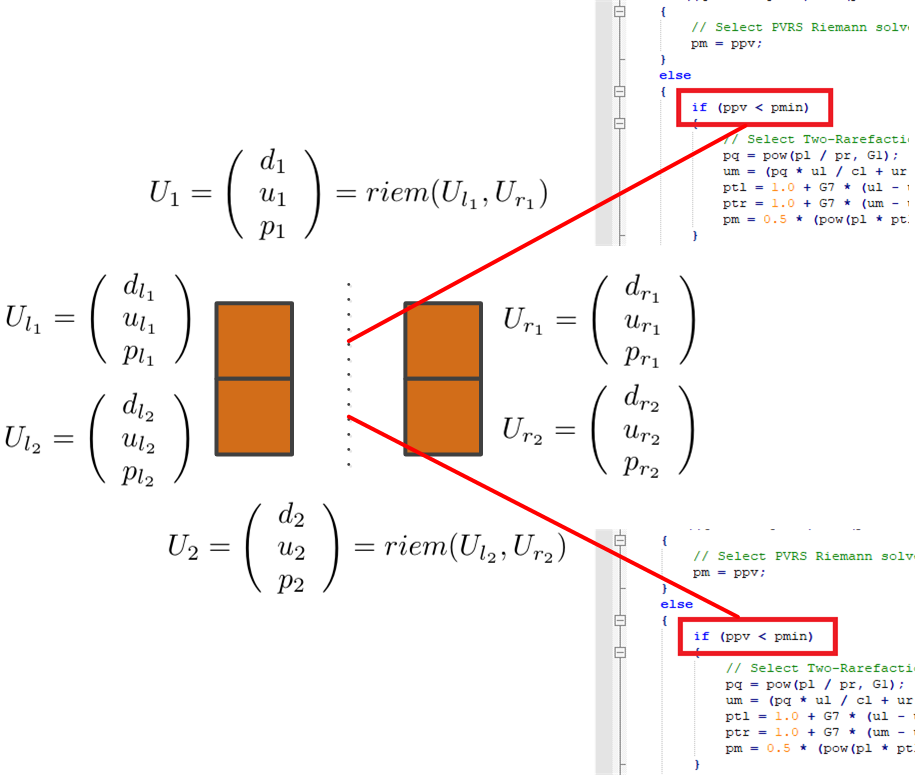
\includegraphics[width=0.6\textwidth]{./pics/text_4_vec_check_mask/continuity.png}
\singlespacing
\captionstyle{center}\caption{Иллюстрация тенденции сохранения значения условия при переходе к соседним ячейками в расчетных задачах.}
\label{fig:text_4_vec_comb_continuity}
\end{figure}

Из этого следует, что и значение условия \texttt{p <= pk} при переходе от одной ячейке к соседней будет изменяться также не слишком быстро.
Но условие это дискретная величина, а это значит, что часто значение условия будет сохраняться при переходе к соседней ячейке.
Рассмотри теоретический краевой случай, когда во время обработки $n$ наборов скалярных данных условие выполняется для первых $np$ из них и не выполняется для оставшихся $n(1 - p)$.
Для простоты будем считать, что все числа $np$, $n(1 - p)$ целые и кратны ширине векторизации $w$.
В этом случае очевидно, что во время выполнения векторной версии кода первые $\frac{np}{w}$ масок \texttt{cond} будут полные, а остальные $\frac{n(1 - p)}{w}$ масок \texttt{cond} будут пустыми (с масками \texttt{ncond} ситуация будет обратной).
В таком случае, время исполнения векторизованной версии кода с проверкой обеих масок \texttt{cond} и \texttt{ncond} на пустоту в точности совпадет со временем $T_1$.
Таким образом, эффективность векторизации в этом теоретически идеальном случае будет ровно единица с поправкой на дополнительные операции проверки масок на пустоту.

Для рассматриваемой функции \texttt{prefun} были собраны расчетные данные распределения плотности маски условия \texttt{p <= pk}, чтобы оценить вероятность появления пустых масок \texttt{cond} и \texttt{ncond}.
На рис.~\ref{fig:text_4_vec_comb_mask_independent_p} слева представлено распределение плотности масок\label{term:vector_mask_density3} в случае независимости условий для разных наборов скалярных данных (нетрудно видеть, что распределение является нормальным).
Результаты распределения плотности маски \texttt{cond}, собранные по настоящему профилю исполнения векторного кода на реальных данных, представлены на рис.~\ref{fig:text_4_vec_comb_mask_independent_p} справа.

\begin{figure}[ht]
\centering
\begin{tabular}{ll}
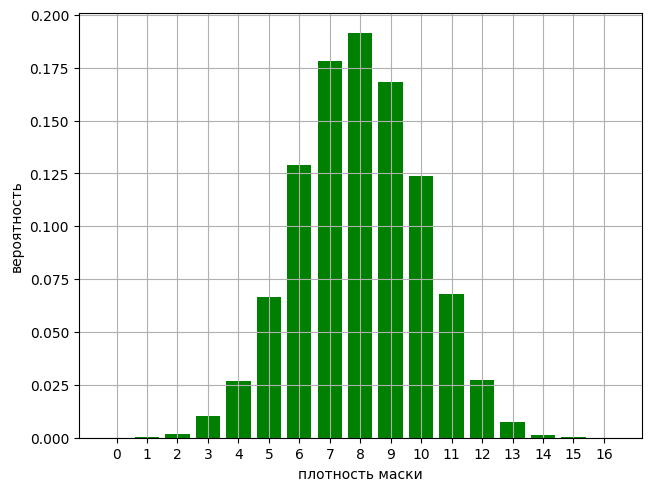
\includegraphics[width=0.45\textwidth]{./pics/text_4_vec_comb_mask/independent_p.png}
&
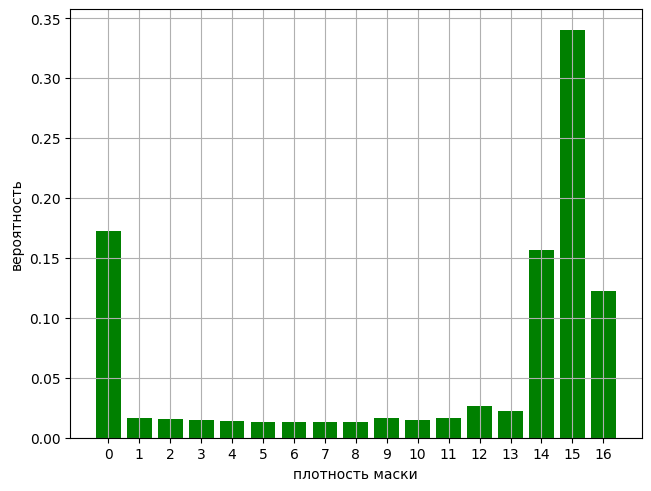
\includegraphics[width=0.45\textwidth]{./pics/text_4_vec_comb_mask/real_p.png}
\end{tabular}
\singlespacing
\captionstyle{center}\caption{Гистограмма распределения плотностей маски \texttt{cond} при условии, что все условия \texttt{p <= pk} для наборов скалярных данных являются независимыми (слева) и на реальном профиле исполнения (справа).}
\label{fig:text_4_vec_comb_mask_independent_p}
\end{figure}

Из рис.~\ref{fig:text_4_vec_comb_mask_independent_p} видно, что распределение плотностей масок на реальных данных совершенно не похоже на распределение, вычисленное в предположении о независимости условий переходов.
Можно заметить, что в реальном коде более четверти всех масок \texttt{cond} являются либо пустыми, либо полными (в этом случае пустой является маска \texttt{ncond}), а значит использование проверок масок на пустоту обосновано.

Для анализа полученных результатов были рассмотрены следующие три подхода к векторизации плоского цикла с условием.
В качестве базового метода векторизация принималось простое слияние путей исполнения под соответствующими предикатами с последующим объединением $w$ последовательных скалярных итераций в одну векторную (простое слияние).
Этот базовый метод сравнивался с двумя рассмотренными выше улучшениями: проверка масок блоков на пустоту (проверка масок) и слияние двух соседних блоков при условии отсутствия пересечения их масок (объединение масок).
Анализ эффективности применения преобразований рассматривался на приведенной в листинге~\ref{lst:text_4_vec_comb_prefun_scalar} функции \texttt{prefun} из реализации газодинамического римановского решателя.\label{term:riemann_solver5}
Профиль исполнения функции собирался на задачах моделирования распада разрыва при различных начальных условиях \cite{Toh2024VecRiemann,Zeng2021VecRiemann}.
Эффективность векторизации при выбранных подходах измерялась двумя способами.
В качестве первого способа использовался режим эмуляции векторных инструкций.
В настоящее время используются различные эмуляторы AVX-512\label{abbr:avx5} с помощью которых можно оценить эффективность\label{term:vec_eff4} векторного кода \cite{Lee2024VecGem}.
При анализе рассматриваемой функции мы ограничились инструментом, позволяющим отследить плотность используемых в коде масок и общее количество скалярных и векторных операций \cite{Rybakov2023VecShvindt}.
Вторым способом сравнения был замер производительности результирующего векторного кода на микропроцессоре Intel Xeon Phi KNL\label{abbr:knl11} 7290.
Результаты сравнения представлены на рис.~\ref{fig:text_4_vec_comb_mask_res}.

\begin{figure}[ht]
\centering
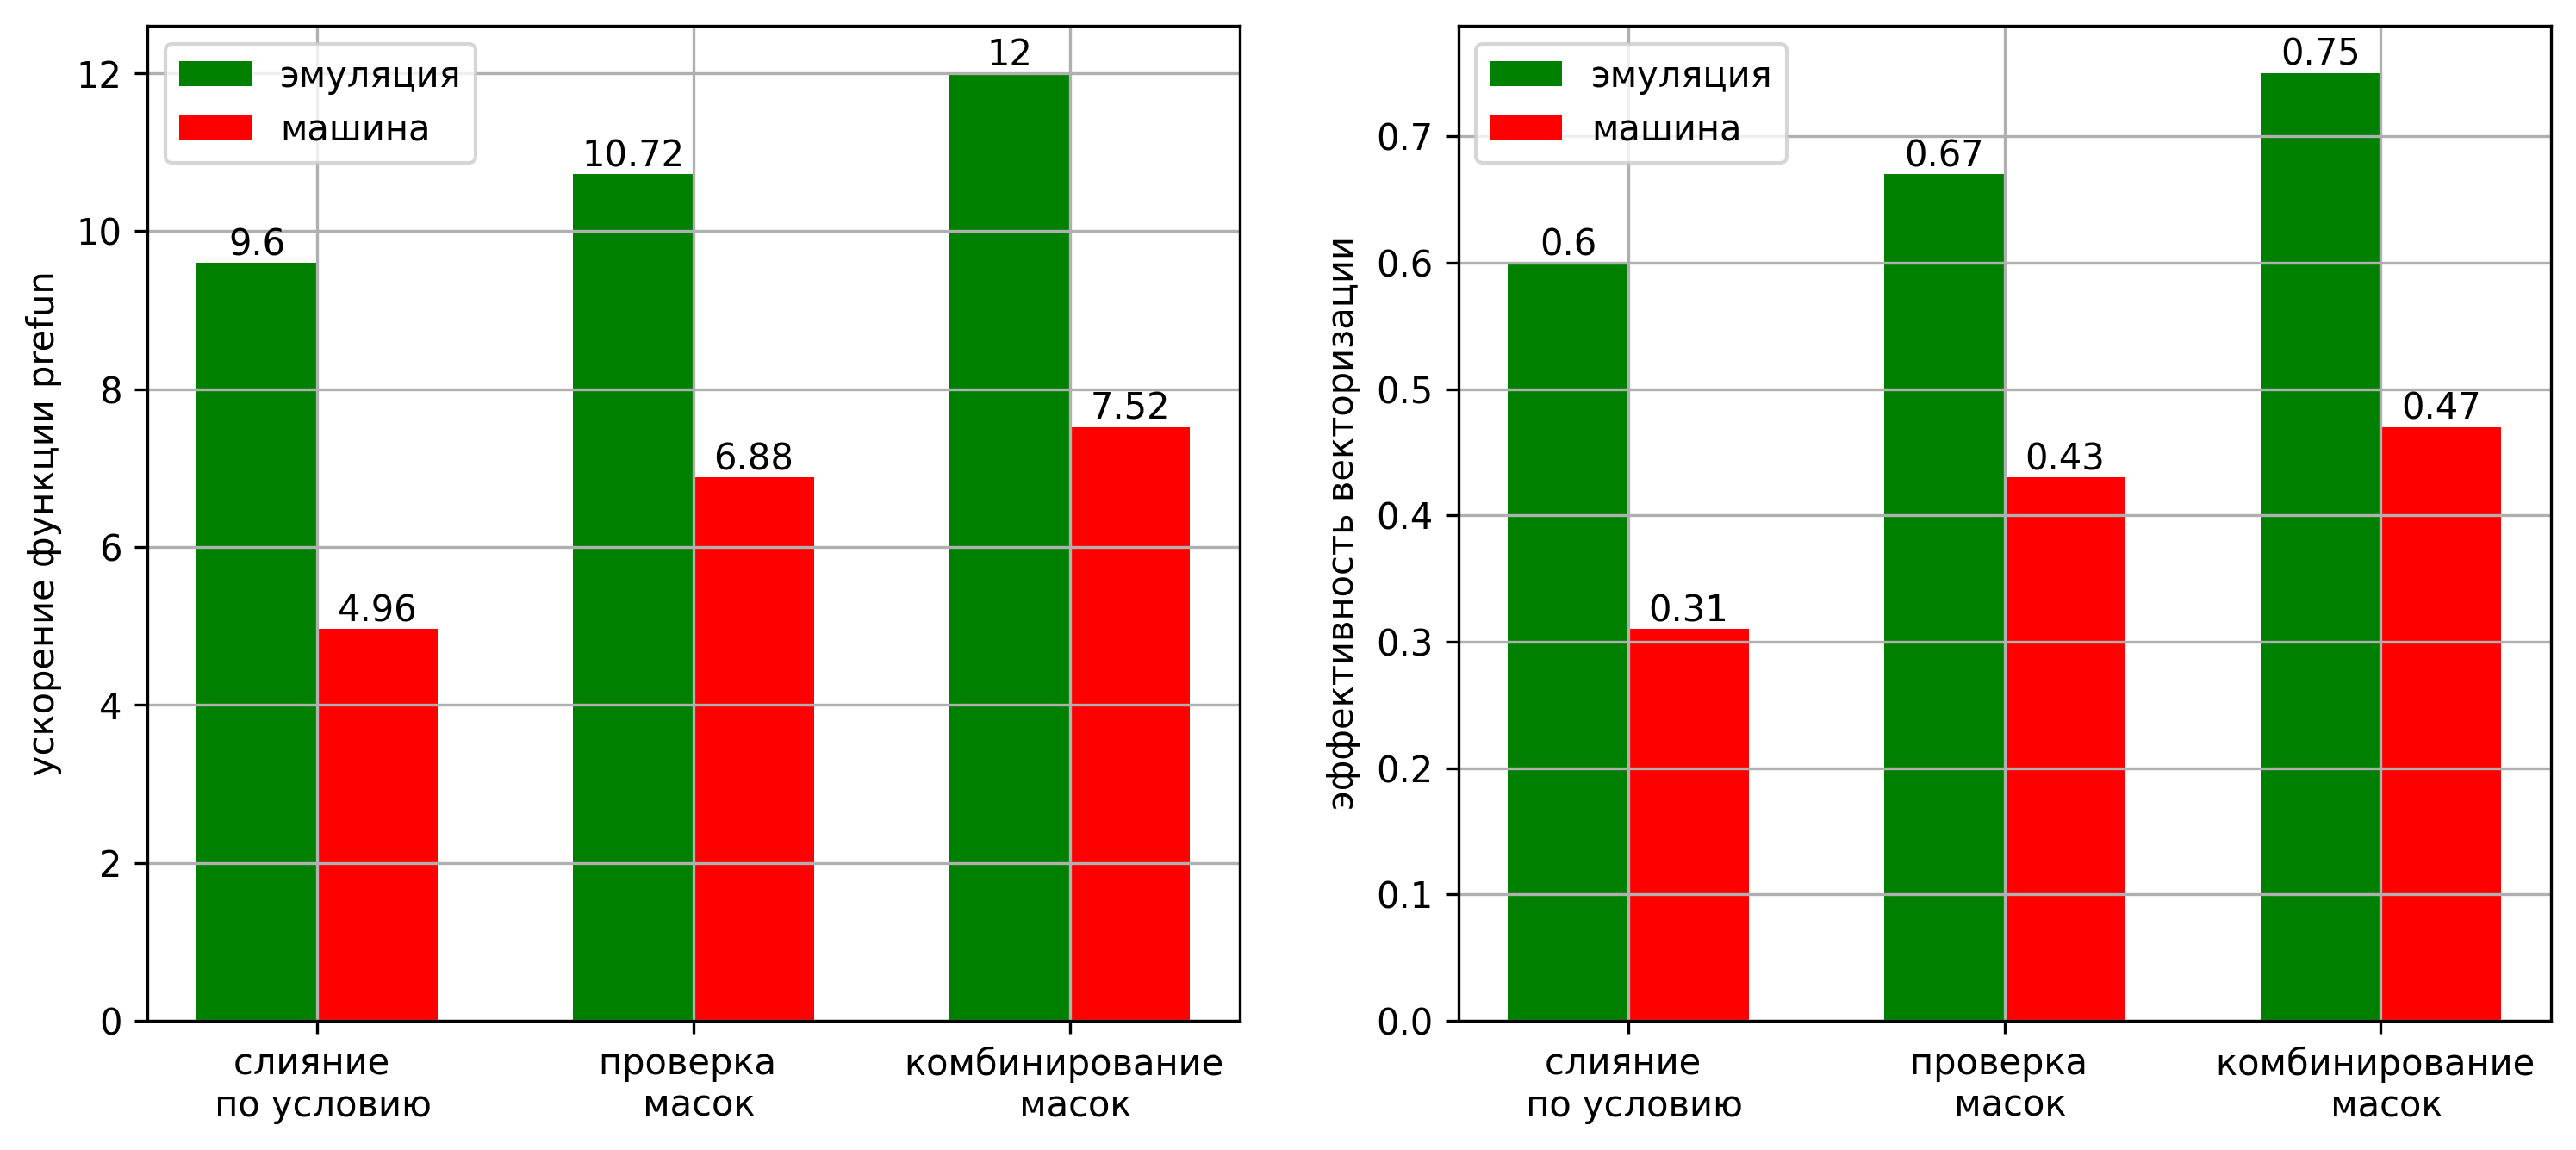
\includegraphics[width=1.0\textwidth]{./pics/text_4_vec_comb_mask/res.png}
\singlespacing
\captionstyle{center}\caption{Результаты сравнения эффективности векторизации при простом слиянии, с проверкой масок и с объединением масок в режимах эмуляции и на микропроцессоре Intel Xeon Phi KNL 7290.}
\label{fig:text_4_vec_comb_mask_res}
\end{figure}

Эксперименты показали, что в режиме эмуляции слияние ветвей исполнения привело к эффективности векторизации 0,6.
Использование дополнительных методов повышения плотности векторных масок в коде -- проверки масок и объединения масок -- привело к повышению эффективности векторизации до показателей 0,67 и 0,75 соответственно.
Эффективность векторизации при проведении замеров на реальной машине оказалась скромнее.
Простое слияние путей исполнения позволило достичь эффективности 0,31, а использование проверок масок и объединения масок позволило повысить эффективность векторизации до 0,43 и 0,47 соответственно.
